\section{Collaboration Projects}

Artificial intelligence and machine learning (AI/ML) are utilized across various components of the CLAS12 experiment, including online data monitoring, offline reconstruction, data analysis, and enhanced particle identification. Their integration into the reconstruction process has led to a substantial improvement in the experiments' statistical precision.

\subsection{AI/ML in CLAS12 tracking}

CLAS12 tracking algorithms employ AI techniques to enhance track reconstruction. A sequence of neural networks operates in concert to maximize efficiency. Initially, a Convolutional Autoencoder is applied to denoise raw signals from the Drift Chambers (DC). Subsequently, a Multi-Layer Perceptron (MLP) connects clusters across the six DC superlayers to identify track candidates. To address inefficiencies such as missing segments in one or more superlayers, a secondary autoencoder is used to recover incomplete tracks. The incorporation of AI into CLAS12 reconstruction has led to a significant increase in tracking efficiency (approximately $20\%$ at a 50 nA electron beam on a hydrogen target), resulting in an estimated $60\%$ gain in collected statistics for three-particle final state reactions.

\begin{figure}[h!]
\centering
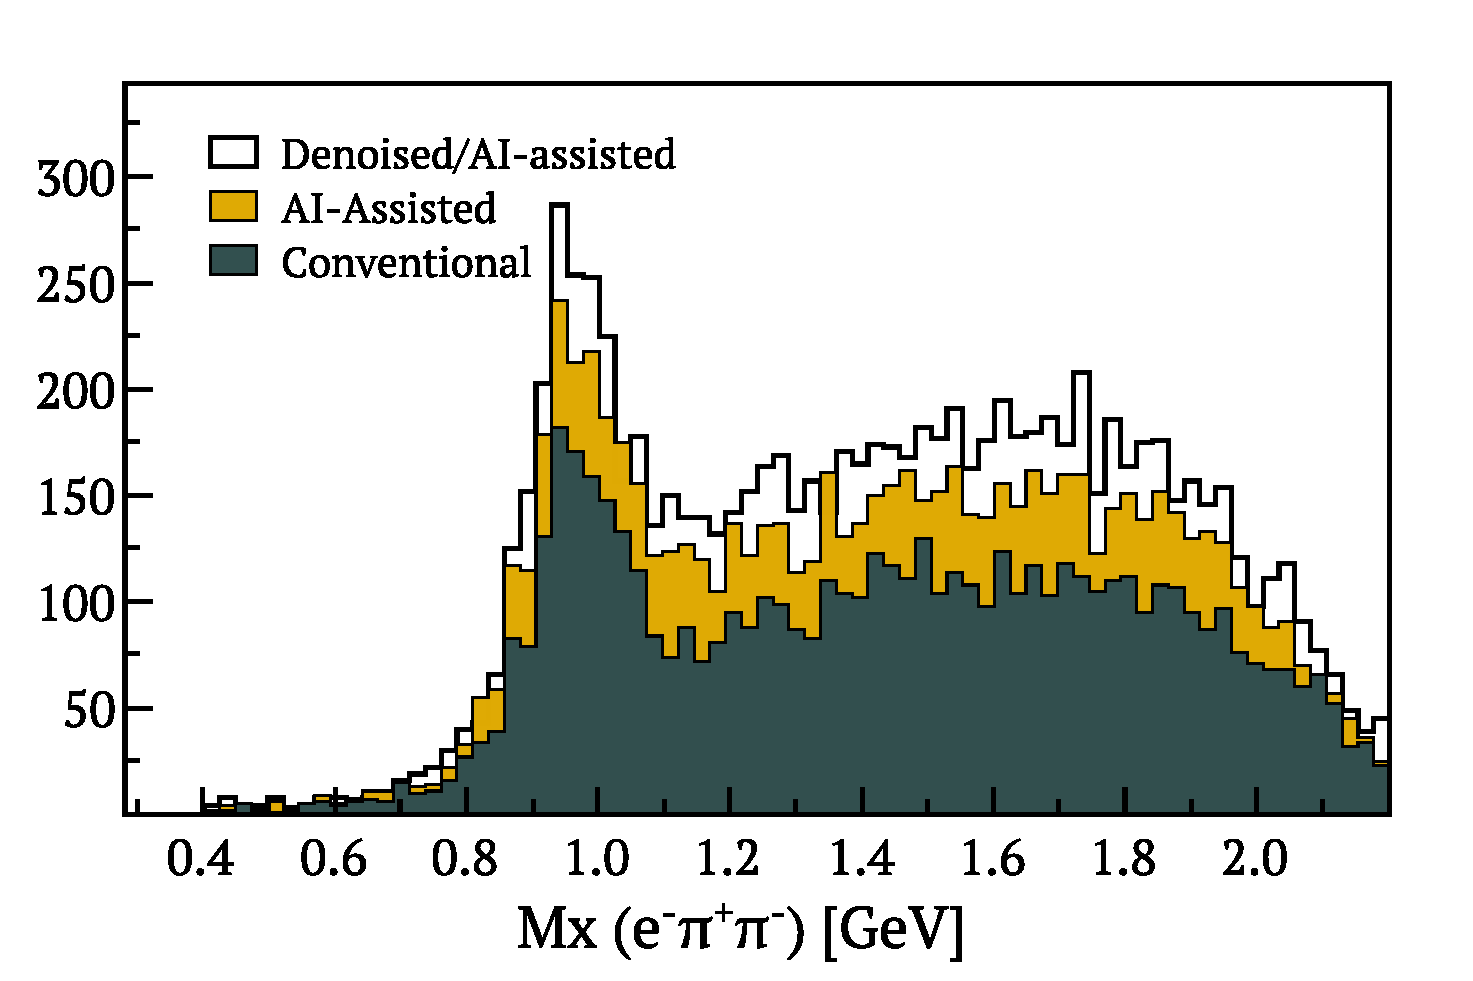
\includegraphics[width=0.42\columnwidth]{images/projects/figure_denoise_mxp.pdf}
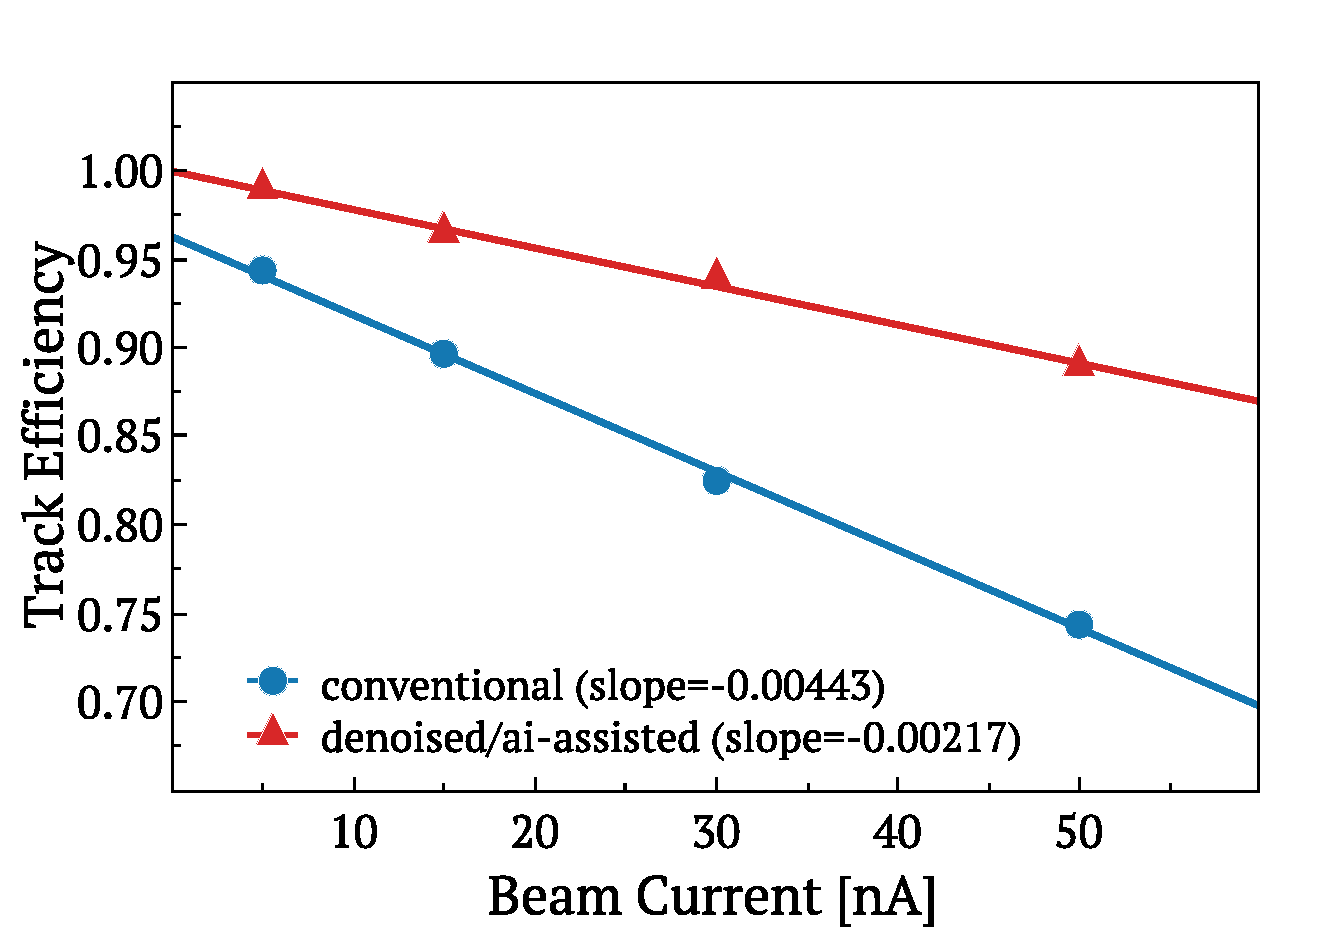
\includegraphics[width=0.42\columnwidth]{images/projects/luminosity_scan.pdf}
\caption{ } 
\label{fig:ai_results}
\end{figure}

Figure~\ref{fig:ai_results} (left) presents the statistical gain for the reaction $H(e) \rightarrow e^\prime\pi^+\pi^-X$, where the missing mass distribution of the detected particles highlights the missing proton. Figure~\ref{fig:ai_results} (right) shows the track reconstruction efficiency as a function of luminosity (beam current), comparing conventional tracking with AI-augmented tracking. The enhanced efficiency achieved through AI integration enables experiments to operate at higher luminosities while maintaining robust track finding performance. AI-augmented track finding has been integrated into the standard data processing workflow and is currently employed in the processing of experimental data.

\subsection{Online Reconstruction in CLAS12}

In the CLAS12 experiment, AI and machine learning techniques are integrated into the online reconstruction workflow, where they operate directly on raw detector signals to identify track candidates and reconstruct tracks in the drift chambers, analogous to traditional offline reconstruction. Neural networks are further employed online to estimate track parameters such as momentum and direction, and to perform particle identification for the reconstructed tracks. The AI-based online reconstruction is optimized for real-time performance and runs at the full speed of the Data Acquisition (DAQ) system.

Given that most CLAS12 experiments involve electron-induced reactions, accurate and efficient electron identification is particularly critical. Figure~\ref{fig:eid} illustrates the performance of the AI-based electron identification. The left panel shows the reconstructed missing mass of the proton for events in which an electron is identified by the online AI algorithm, compared to those identified using the conventional reconstruction. The AI-based approach yields a $30\%$ increase in the number of identified events, highlighting a significant statistical gain over the traditional methods.

\begin{figure}[h!]
\centering
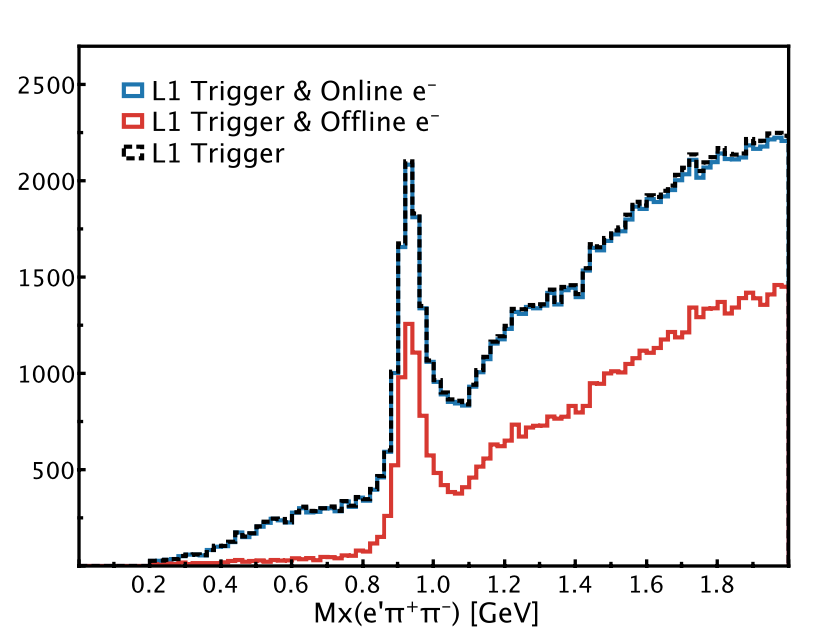
\includegraphics[width=0.42\columnwidth]{images/projects/level-3-eid.png}
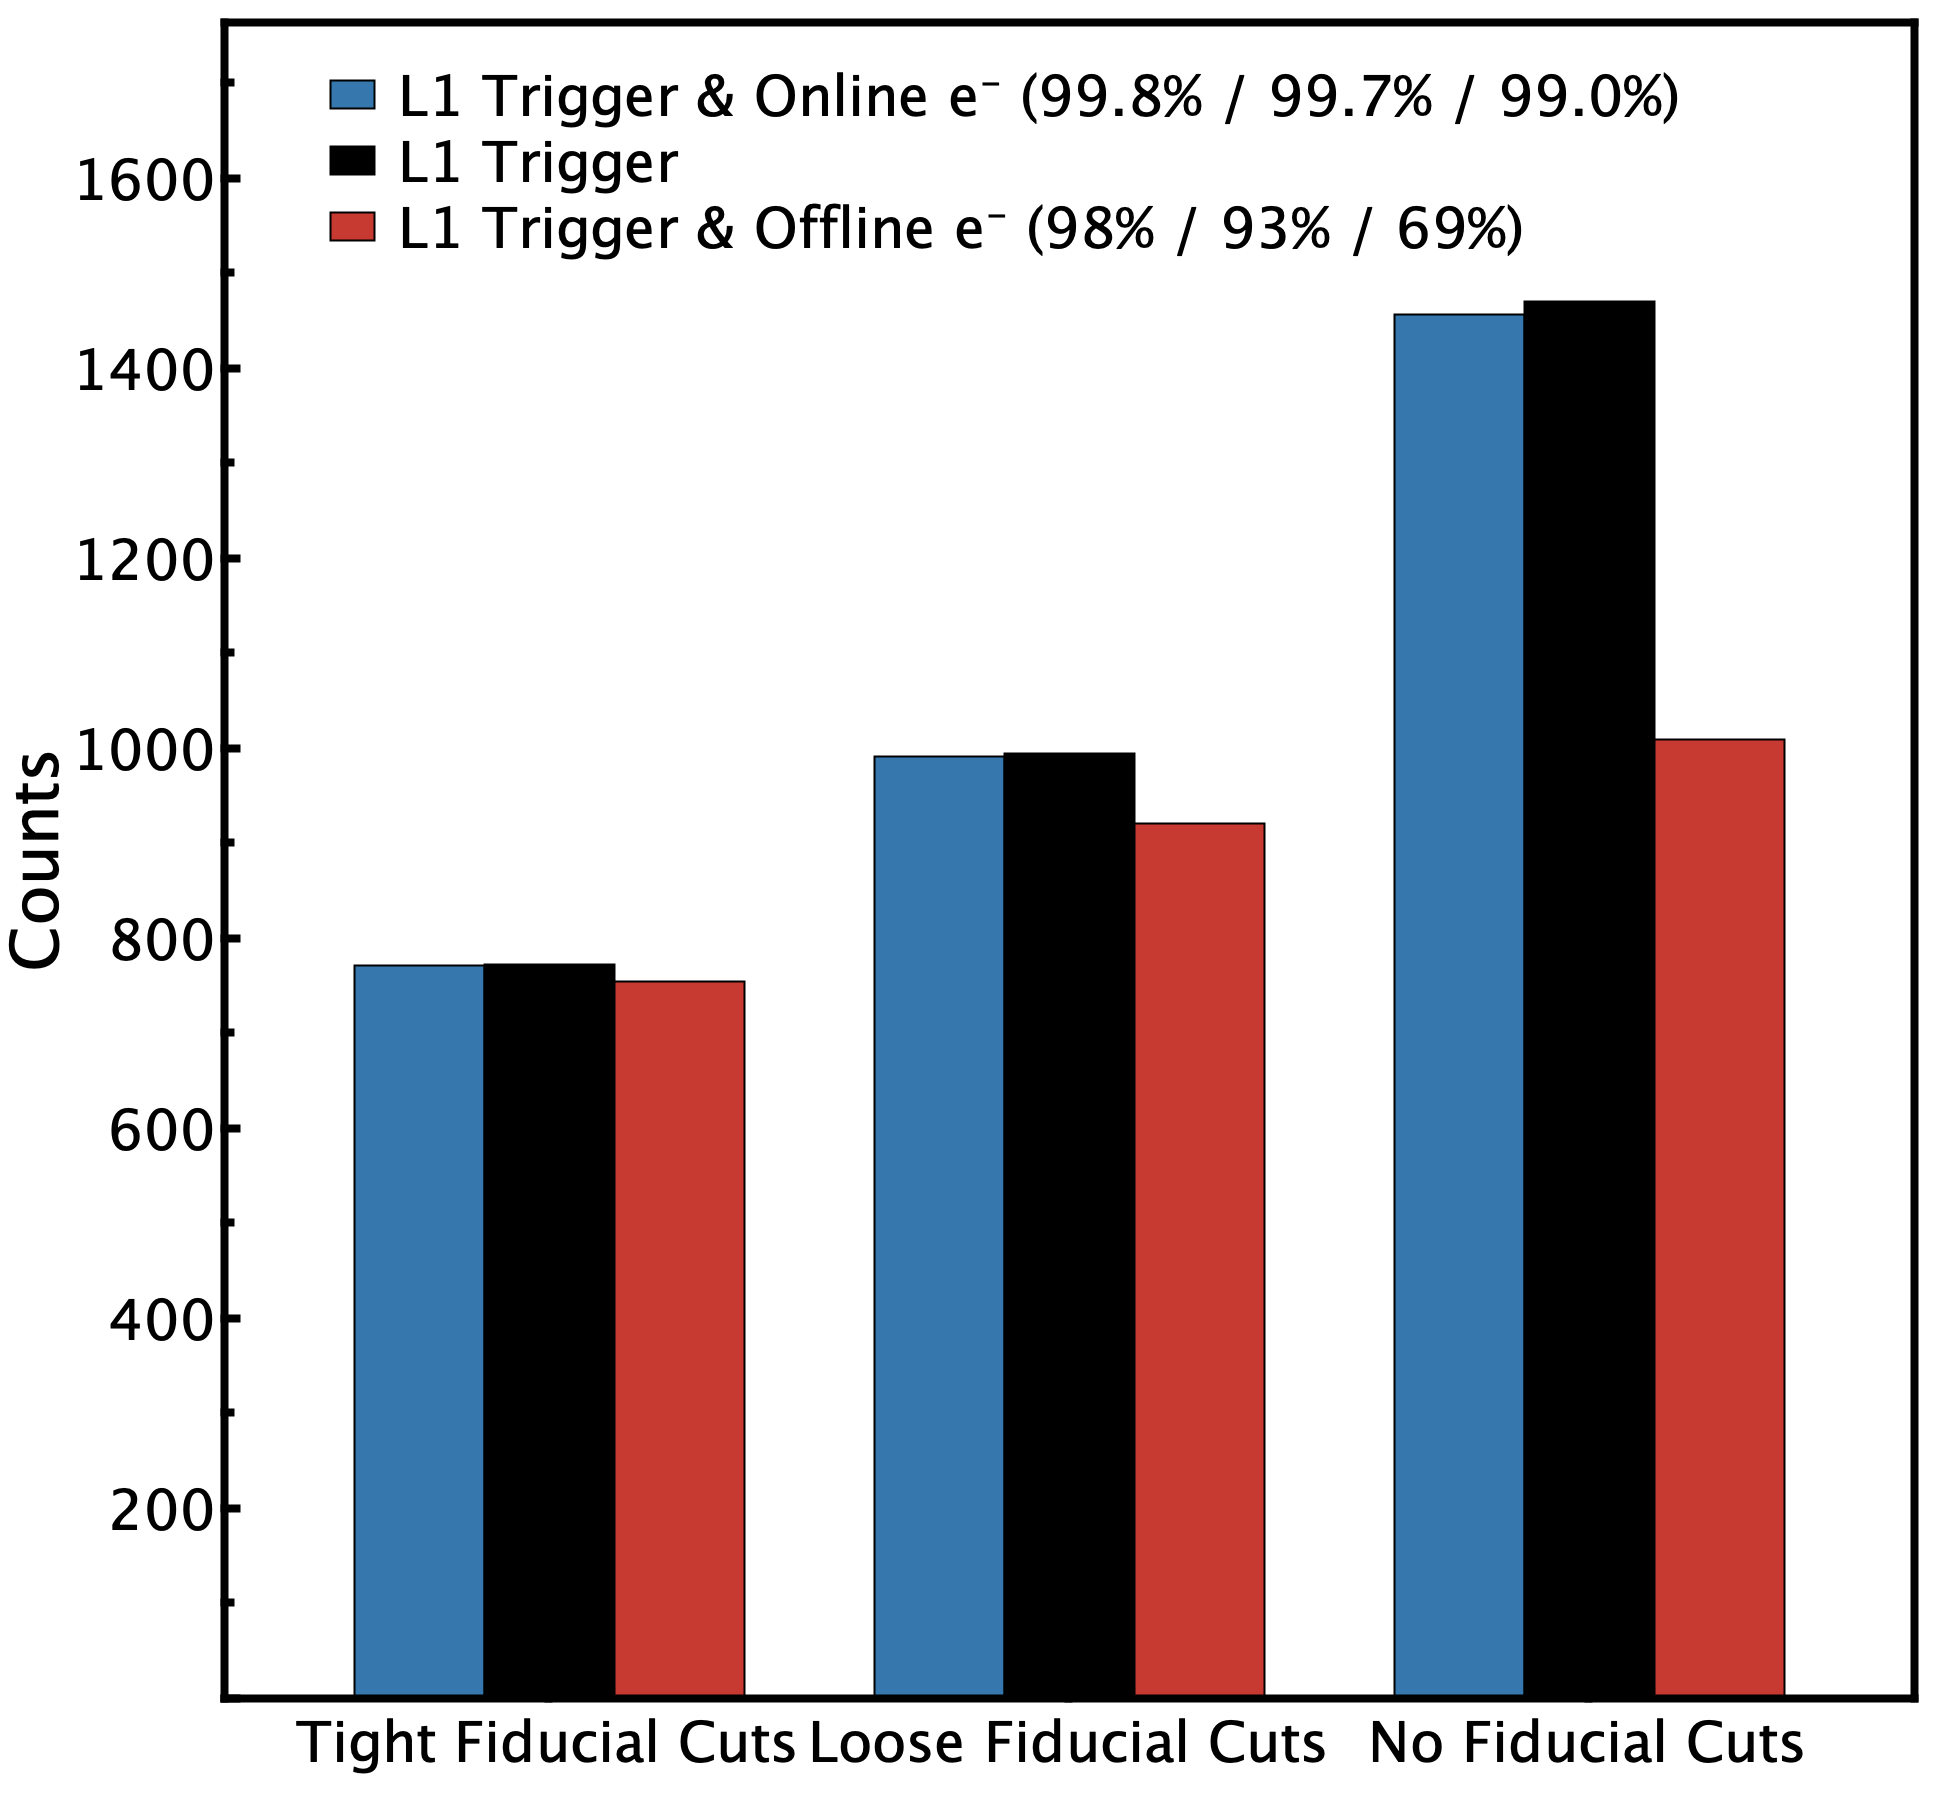
\includegraphics[width=0.32\columnwidth]{images/projects/epipiRad_barchart.png}
\caption{AI/ML electron identification compared to conventional offline algorithms. (left) The missing mass of $H(e) \rightarrow e^\prime\pi^+\pi^-X$ is shown for conventional and AI electron identification, showing a significant increase in statistics in the missing proton peak. (right) The improvement of electron identification is shown as a function of cuts on the fiducial region of the EC.} 
\label{fig:eid}
\end{figure}

In Figure~\ref{fig:eid} (right panel), the improvements in electron identification are shown across different regions of the Electromagnetic Calorimeter (EC). The fiducial region refers to areas well within the EC boundaries, whereas regions near the edges are more prone to partial shower containment, where the electromagnetic shower produced by an electron may escape the detector. This leads to reduced energy deposition, making electron identification more challenging for conventional algorithms. AI-based algorithms, however, can be trained to recognize such incomplete signatures and successfully recover these events, resulting in a notable increase in statistics from experimental data.
The capability to reconstruct tracks and identify electrons in real time is essential for the CLAS12 detector's transition to a trigger-less Streaming Readout (SRO) system, where large volumes of data must be processed on-the-fly to select and preserve only the most relevant events.

\begin{figure}[h!]
\centering
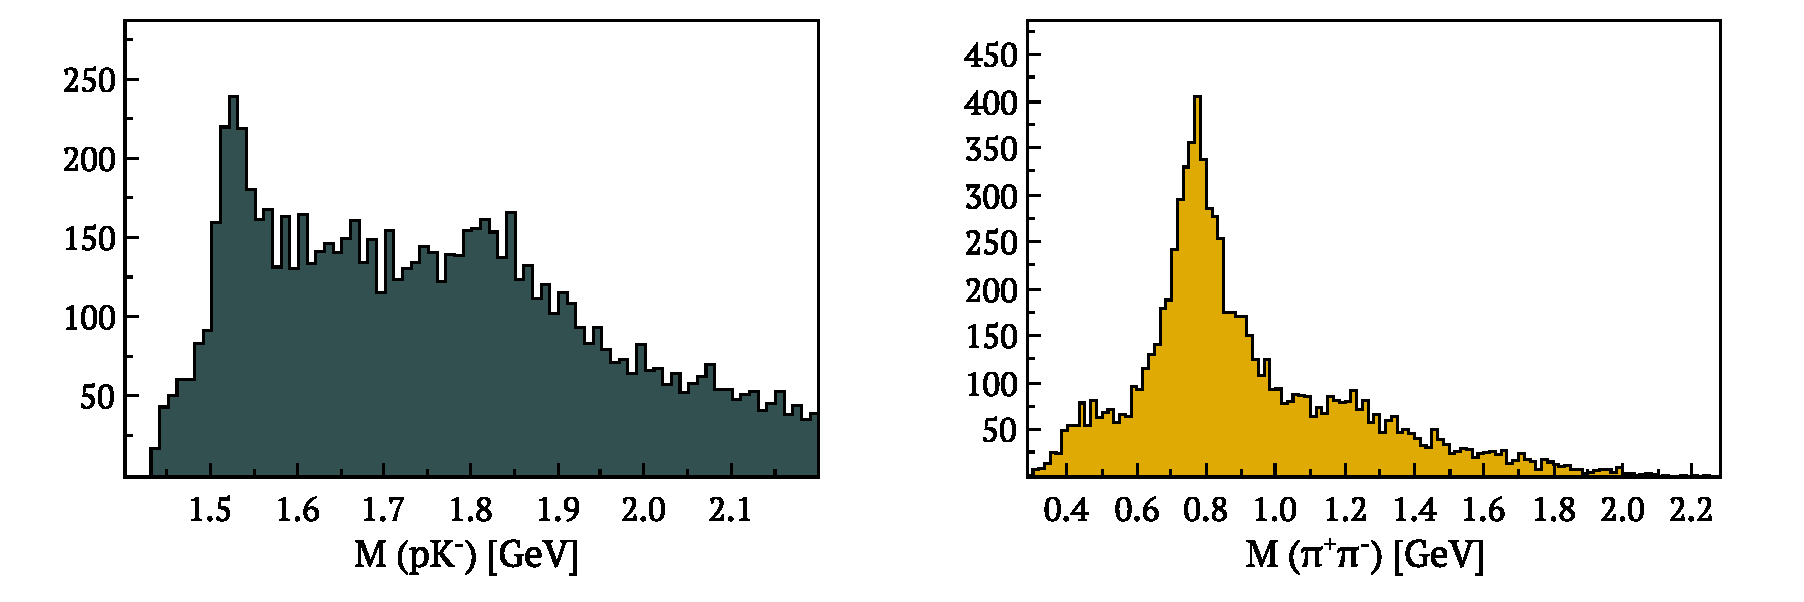
\includegraphics[width=0.95\columnwidth]{images/projects/figure_lambda_instarec.pdf}
\caption{Identified physics decay states from online AI/ML reconstruction. (left) the invariant mass of $K^+p$ with selection of $e^\prime K^+p(K^-)$, with $\Lambda$ peak around 1520 MeV. (right) invariant mass of $\pi^+\pi^-$ with $\rho(770)$ peak visible. } 
\label{fig:physics}
\end{figure}

Furthermore, reconstructed tracks with identified electrons can be used to determine the reaction channel for each event and to compute physics observables in real time. Figure~\ref{fig:physics} presents invariant mass distributions for two such identified reactions. In the left panel, the reaction $e^\prime K^+p X$  is shown, where the missing mass analysis identifies $X$ as $K^-$, and the resulting $K^+p$ invariant mass distribution reveals the presence of the $\Lambda(1520)$ resonance.
In the right panel, the invariant mass of the  $\pi^+\pi^-$ system is plotted for identified $e^\prime \pi^+\pi^- (p)$ events, clearly showing the reconstructed $\rho(770)$ resonance.
In the physics results shown, the particles, including the momentum and direction, are reconstructed from raw experimental data using AI at speeds higher than data acquisition rates. 

The integration of AI/ML methods into CLAS12 reconstruction algorithms has significantly enhanced the physics output of the experiments. Moreover, the development of full AI-based event reconstruction marks a transformative shift in data processing for nuclear physics, enabling real-time physics analysis during data acquisition. This capability to identify reaction channels as data is collected allows for the selection of specific event topologies on-the-fly, substantially reducing post-processing time and accelerating the timeline from data collection to publication.



